% !TEX root = ../Dissertation.tex
%===================================================================================================

\chapter{Background}


\section{Type 1 Diabetes - Facts and Figures}
\label{sec:sectionLabel}


Diabetes mellitus is a condition affecting the body's ability to control blood sugar levels.
There are two kinds of diabetes mellitus, type 1 and type 2.
Type 1 Diabetes (T1D) is a serious autoimmune condition whereby the body's own immune system destroys the insulin producing beta cells in the pancreatic Islets of Langerhans \citep{Daneman2006}.
Type 2 Diabetes, however, is a condition where the body becomes either resistant to insulin or the insulin producing beta cells become dysfunctional.
Whereas T1D is an antoimmune disease with typical onset during adolescence, T2D is more prevalent in older people and is linked to changes in lifestyle \citep{OxClinMed}.
This project is concerned with T1D and it's autoimmune basis.

According to statistics provided by Diabetes UK, diabetes, both T1D and T2D, affects approximately 3.9 million people in the UK, with many more as yet undiagnosed. 
Of all diabetes sufferers, around 10\% have T1D \toref{Diabetes UK 2015}.

Insulin is a vitally important hormone involved with the maintenance of normal blood glucose levels, in particular stopping dangerous rises in blood glucose levels.
Insulin's main actions are to stop the production of extra glucose when blood glucose is already sufficiently high.
It does this by keeping the brakes on gluconeogenesis, glycogenolysis, lipolysis, ketogenesis and proteolysis, and preventing the production of glucagon, the hormone which acts to raise glucose levels.
However, in T1D, the resulting lack of insulin means that these processes cannot be kept in check causing subsequent hyperglycaemia \citep{Sonksen2000}.
The total lack of insulin production ability in T1D means that effective glucose monitoring and self administration of glucose via injection or infusion is cruicial to maintain blood glucose homeostasis.

Alongisde the charactistic symptoms of excessive thrist, drinking and urination, there are serious side effects both in the short and longer term.
In the short term, extremes of blood glucose, either too high or too low can lead to hyper- or hypoglycaemia which can prove lethal if not treated promptly.
In the longer term, prolonged mild hyperglycaemia caused by T1D can cause micro- and macrovascular complications leading to blindness, neuropathy, kidney failure and a significantly increased risk of cardiovascular disease\citep{OxClinMed}.
It is therefore vitally important for research into T1D to continue, with the aim of finding a cure.

There are currently two arms of T1D research.
The first involves using diabetic patients.
This has it's limitations due to the lack of tissue availability and because a lot of the beta cell destruction occurs prior to the appearance of T1D symptoms \citep{Thomas2000}.
The other arm requires the use of animal models, particularly the nonobese diabetic (NOD) mouse, which is currently the best available animal model of T1D.
The NOD mouse will be discussed further below.

\section{The Nonobese Diabetic Mouse}

The nonobese (NOD) mouse is the best available animal model of T1D, first developed by Makino et al \toref{Makino et al 1980} in 1980.
It is a model that is genetically predisposed to develop T1D by a well characterised pathogenesis over a well defined time course as outlined below and in \cref{fig:diseasecourse}.

\begin{figure}
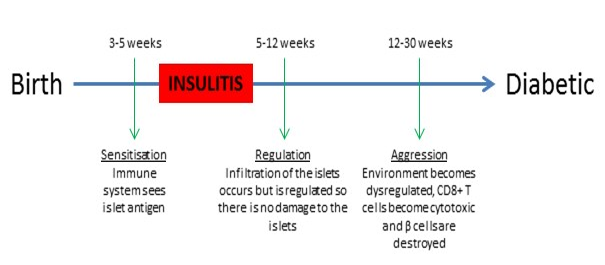
\includegraphics[width=\textwidth]{Figures/Diseasecourse.png}
\caption{Figure showing the T1D process in the NOD mouse.}
\label{fig:diseasecourse}
\end{figure}

\begin{enumerate}
\item Sensitisation - the immune system first becomes aware of islet antigen and incorrectly recognises it as foreign
\item Infiltration and insulitis - cells of the immune system move to the pancreatic islets and infiltrate the tissue. This is known as insulitis. For a while, the environment remains regulated and no damage occurs
\item Beta cell destruction - activated cytotoxic T cells (CTL) begin to target and destroy beta cells. Beta cells are believed to die by apoptosis \citep{Cnop2005}.
\end{enumerate}

It is believed that the NOD mouse is a relevant model for T1D research as it is thought the human disease follows a similar pathogenesis.
It has been seen in donated human diabetic tissues that there is infiltration of islets including many CD8\textsuperscript{+} T cells, suggesting that they may well be activating to cytotoxic T lymphocytes (CTL) and destroying $\beta$ cells in a similar way to that seen in the NOD mouse \citep{Hanafusa2008}.
Each of the stages of T1D development will be discussed further in the relevant sections below.


\subsection{Initiation of T1D}

It is not known what causes T1D.
There are numerous hypotheses as to how the immune system first becomes aware of islet antigens that normally remain hidden.

One such hypothesis is that a childhood illness affecting the pancreas may cause release of islet antigen in an inflammatory environment \citep{Green1999, Andreoletti1997}.
The inflammatory environment would mean that antigen presenting cells (APCs) would be expressing co-stimulatory molecules (see \cref{subsec:Tcellactivation}) so they would be able to activate T cells responsive to islet antigen released.
This could then allow T cell-mediated $\beta$ cell destruction.
However, this model for human disease would not fit with the disease seen in the NOD mouse as the highest incidence of T1D is seen in colonies housed in specific-pathogen-free facilities\citep{Delovitch1997}.
This means the mice would not have had the same virus exposure to trigger the disease and yet T1D is observed anyway.

Another possibility may involve the normal physiological process of pancreatic remodelling during growth and development.
Normally this occurs in a non-inflamed environment and as cells die an d are replaced, the debris is cleared up by macrophages.
The lack of inflammatory signals means that APCs do not become activated and therefore cannot present to T cells and mount an immune response \citep{Green1999}.
However, if there is inflammatory signalling, or presence of inflammatory cytokines, the APCs are able to activate T cells and ellicit an immune response.
This could suggest that the NOD mouse may be remodelling its pancreas in a more inflammatory environment, allowing the activation of APCs.
Support for this theory was provided by the production of a TNF$\alpha$-NOD mouse, whereby TNF$\alpha$ is expressed in the islets.
The presence of this inflammatory cytokine sped up the onset of diabetes and it was seen that some beta cells apoptosed prior to DC infiltration and that the DCs became activated\citep{Green1998}.

Autoantigens believed to be important in T1D are glutamic acid decarboxylase (GAD), insulin, islet-specific glucose-6-phosphatase catalytic subunit-related protein (IGRP) and insulinoma antigen-2 and 2$\beta$ \citep{Green1999, Roep2012}.


\subsection{Infiltration and Insulitis}

Following sensistisation to islet antigen, immune cells then begin to move into the islets to form an infiltrate.
First only the edges of the islets are affected and this is known as peri-insulitis\citep{Thomas2000}.
However, soon cells move into the islets too.
Cells involved are DCs, macrophages, B cells and T cells\citep{Brodie2008}.
It is believed that insulitis is the point at which tolerance to beta cell antigen is lost \citep{Thomas2000}.
There is evidence to suggest that this pathogenesis is not limited only to the NOD mouse as pancreatic samples from diabetic humans also reveal infiltrated islets.
As mentioned above, this infiltrate contains CD8\textsuperscript{+} T cells, which have potential to become CTLs, other lymphocytes and APCs \citep{Hanafusa2008}.

\subsection{Beta cell destruction}

Following non-destructive insulitis, immune cells gain their aggressive traits and beta cells begin to be destroyed.
The destruction of beta cells in NOD and human pancreatic islets is believed to be mediated by cytotoxic T lymphocytes (CTLs)\citep{Thomas2000, Brodie2008, Hanafusa2008}.
The destruction of beta cells in T1D leads to absolute insulin deficiency \citep{Daneman2006}.

\section{B cells}
\subsection{Role of B cells}
\label{subsec:Bcellrole}
B cells have two physiological roles, antigen presentation and antibody production.
Whilst B cells are APCs, their main function is antibody production.
Antibodies are an important part of the adaptive immune response which help with the neutralisation of toxins, phagocytosis of pathogens and destruction of bacteria and viruses.

B cells also play an important role in the pathogenesis of T1D. 
This will be discussed in more detail in \cref{sec:BcellsinT1D}

\subsection{Development - Stem cells to maturity}
\label{subsec:Bcelldevelopment}
\subsubsection{B cell commitment}

Haematopoietic stem cells are the progenitors from which all blood cells derive.
These cells are found in the bone marrow and, via the production of various progenitors, can produce megakaryocytes, erythrocytes, lymphocytes, granulocytes, macrophages and natural killer cells.
HSCs are characterised by their Lin\textsuperscript{-} Sca\textsuperscript{high} c-kit\textsuperscript{high} expression (So called LSK cells) and lack of surface Flt3\citep{Welinder2011}.

Following the haematopoietic stem cell stage, multipotent progenitors form which have the capability of producing all types of blood cell, but lack the self-renewing ability of HSCs \toref{Ref for this}.
These cells are LSK but also express Flt3\textsuperscript{low} \citep{Welinder2011}.
Interestingly, MPPs can express genes of multiple lineages \citep{Hu1997} suggesting that this expression is due to priming for lineage committment, rather than commitment itself.
It is thought that by expressing these genes, it maintains them in an accessible chromatin state, ready for commitment \citep{Welinder2011}.
Evidence for this has been seen through changes in chromatin staus of lineage restricted genes during blood cell development \citep{Weishaupt2010}.

Following MPP development, magakaryocytic and erythrocytic potential is much reduced and the so-called lymphoid primed multipotent progenitor (LMPP) arises.
These cells are capable only of lymphocyte, macrophage, granulocyte and NK cell production \citep{Adolfsson2005}.
LMPPs are characterised by being LSK but also Flt3\textsuperscript{high}.

Next, Il-7R$\alpha$ upregulates and Sca-1 and c-kit downregulate and to form common lymphoid progenitors (CLP).
These cells are capable only of B and T lymphocyte development and NK cell development \citep{Kondo1997} and are Sca-1\textsuperscript{low} c-kit\textsuperscript{low} Flt3\textsuperscript{+} Il-7R$\alpha$\textsuperscript{+}.
Flt3 is the receptor for Flt3 ligand (Flt3L) which is found in the bone marrow and acts as a growth promoter for CLPs.
Flt3L also works synergistically with IL-7 to promote lymphocyte proliferation \citep{Holmes2006}.

However, further research into CLPs has revealed significant heterogenity within the population.
Many different groups have used different methods, markers and reporters in order to try and identify a subpopulation of CLPs which is restricted to the B cell lineage. 
Some of these are outlined below:
\begin{itemize}
\item \citet{Mansson2010} - Expression of $\lambda$5 and Rag1 was used to divide the CLP compartment into cells that are able to produce T, B and NK cells, cells that are able to produce T and B cells, and those that are B cell restricted.
Using $\lambda$5 reporter mice crossed with Rag1 reporter mice, it was found that CLPs could be divided into three populations.
$\lambda$5\textsuperscript{-}Rag1\textsuperscript{low} cells which produced T, B and NK cells, L5\textsuperscript{-}Rag1\textsuperscript{high} which produced T and B cells with reduced NK cell potential, and $\lambda$5\textsuperscript{+}Rag1\textsuperscript{high} cells which were B cell lineage restricted.
They also found that the $\lambda$5\textsuperscript{high}Rag1\textsuperscript{high} cells had increased expression of the surface marker Ly6D.
\item \citet{Inlay2009} - Expression of Ly6D was used as a marker for determining B cell lineage commitment.
For their investigations they split CLPs into Ly6D\textsuperscript{+} and Ly6D\textsuperscript{-} fractions and then looked at their ability to produce T, B and NK cells.
Interestingly, Ly6D\textsuperscript{-} CLPs were able to produce all three types of progeny and were therefore termed all-lymphoid progenitors, ALPs.
On the other hand, Ly6D\textsuperscript{+} CLPs were almost totally B cell committed.
\item \citet{Zhang2013} - Expression of Ly6D and Rag1 were used as markers to follow B cell commitment and differentiation.
The CLP compartment was split based on Flt3 expression, Rag1 expression and Ly6D expression.
It was found that those cells expressing Ly6D and Rag1 were the most potent at producing B cells. 
Most of these cells also expressed Flt3.
These B cell producing cells also had the highest levels of B cell gene Rag1, EBF and pax5 transcripts (for example, Rag1, EBF, Pax5, see \cref{subsec:Bcellgenes} indicating B cell lineage progression.
\end{itemize}

It therefore appears that within the CLP stage, there are subpopulations of cells which have leanings towards different lineages.
It may be that the appearance of these different subpopulations is linked to the developmental stage of the CLP.
For example, the more committed progenitors, like BLPs, might be more developed CLPs compared to less committed progenitors, such as ALPs.
It appears that Rag1 and Ly6D are very important in determining B cell restricted progenitors and that it is reasonable to hypothesise that a committed B cell progenitor (BLP) could have the phenotype of Sca-1\textsuperscript{low} c-kit\textsuperscript{low} Flt3\textsuperscript{+} IL-7R$\alpha$\textsuperscript{+} Ly6D\textsuperscript{+} with evidence of previous Rag1 expression and robust levels of B cell development gene transcripts.

Following the development of B cell comitted progenitors, these cells then go on to express B220 (expressed on B cells and some plasmacytoid DCs), followed by CD19.
Originally it was thought that B cells were only committed to the B cell lineage once B220 and CD19 were being expressed, however, there is now much evidence to suggest that this committment step occurs prior to their expression.


\subsubsection{Committed B cell development}

Following commitment to the B cell lineage and the expression of CD19, B cells then progress through the following stages \citep{Cambier2007}:
\begin{itemize}
\item Pro B cell - CD19+CD43+IgM-
\item Pre B cell - CD19+CD43-IgM-
\item Immature B cell - CD19+CD43-IgM+
\end{itemize}

For progression from the pro B cell stage to the pre B cell stage, pro B cells must begin the rearrangement of their IgM heavy chain (see below).

Following the production of immature B cells in the bone marrow,they then leave the bone marrow and migrate to the spleen to mature.
This is facilitated by the increase in IgM expression during development which allows immature B cells to become transitional B cells and migrate towards the centre of the bone marrow. 
From here they are carried by the central sinus then venous circulation to the spleen \citep{Loder1999}.


\subsubsection{B cell receptor development}
\label{subsubsec:Bcellrecepdevelopment}

The B cell receptor is the B cell's way of identifying pathogens in a very specific manner.
This means that each B cell must have a different BcR in order to have repertoire capable of recognising different antigens.
In order to produce such a highly diverse repertoire, there are a few mechanisms in place during B cell development which allow the production of a highly diverse BcR across B cells.

The structure of a BcR consists of 2 heavy chains, which have a constant region and a variable region.
Alongside these are two light chains, which also consist of a constand and variable region.
The each light chain sits alongside the heavy chain with the two variable regions next to each other.
Between them, the variable regions make up the antigen binding site.
The constant regions give the antibody its class, for example, IgM, IgD, IgE, IgA, IgM \citep{Pieper2013}.

For both heavy and light chains, the variable region is made up of a V (variable), D (Diversity, heavy chain only) and J (joining) gene segments. 
Genomically encoded are multiple copies of different V, D and J genes and during rearrangement, one of each of these genes are selected at random and joined to produce different combinations of receptors.
This process is mediated by recombinase enzymes encoded by the recombination activating genes (RAG) and are therefore known as rag recombinases.
These enzymes recognise recombination signal sequences (RSS) found next to the coding regions of each V, D and J gene and bring the ends of the chosen genes near to each other to be joined \citep{Fugmann2014, Oettinger1999}.
To join the segments, RAG proteins cleave at either end of the genes and leave hairpin loops of DNA.
From here a nuclease nicks the loops leaving short sequences at the end of each gene to be joined.
This allows the segments to join via non homologous end joining \citep{Schatz2011}.
Further diversity is also added via the use of an enzyme called terminal deoxynucleotidyltransferase (TdT) which adds random base pairs between each segment.
The use of TdT allows the production of the ~10\textsuperscript{14} different immunoglobulins \citep{Motea2010}.

In order to progress from the pro B to the pre B cell stage, the rearrangement of the IgM heavy chain must begin.
Once this has happened, it can be coupled to a surrogate light chain to form the pre-BcR which has the role of initiating light chain rearrangement so that a full IgM molecule can be produced \citep{Burrows2002}.
The transition from pro B to pre B cells is also the first point of screening for autoreactivity\citep{Pieper2013}.

The BcR may either be membrane bound or secreted in the form of antibody.
Antibodies are produced by B cells that have differentiated into plasma cells and are secreted into the blood stream to help with pathogen toxin neutralisation, phagocytosis and complement activation\citep{Janeway2008}.


\subsection{Genes and Transcription Factors driving B cell development}
\label{subsec:Bcellgenes}

The process of B cell development is reliant on the expression of particular genes and transcription factors.
The matter is complicated by the non-linear action of these factors, they all act to regulate each other and work together to drive B cell development \citep{Mandel2010}.

PU.1 is an important transcription factor which requires repression in order to allow B cell development \citep{Dekoter2000}. 
Without this repression, myeloid cell development is encouraged, therefore PU.1 is said to act in a dose dependent manner.
PU.1 is regulated by Gfi-1, which is controlled by Ikaros, a transcription factor known for it's importance in allowing B cell development \citep{Yoshida2006, Busslinger2004}. 

Lowered expression of PU.1 upregulates the expression of IL-7R$\alpha$, EBF and Pax5 which are all important factors for B cell development \citep{Hagman2006}.
PU.1 acts on progenitors in order to aid production of CLPs \citep{Hagman2006}.

Downstream from CLPs, other factors such as E2A, EBF and Pax5 all become important in the commitment to and progression in the B cell lineage \citep{Mansson2008}.
E2A encodes two transcription factors, E12 and E46, both of which are important for B cell development \citep{Bain1997}, shown by the developmental block at the pre-pro B cell stage in the absence of E2A \citep{Bain1994}.
E2A is also a requirement for the expression of EBF-1, which in turn activates genes crucial to BcR development, such as VPreB (a surrogate light chain) \citep{Welinder2011}.
Alongside gene activation, Ebf-1 also activates the transcription factor FOXO-1 which is important for continued B cell development and Rag expression\citep{Amin2008}.

Pax5 is also an important transcription factor.
Originally, it was believed to be the factor that coincided with B cell commitment, however, there is now evidence to suggest that B cell commitment occurs prior to Pax5 expression \citep{Mansson2008}.
It is now thought that Pax5 is important for progression in the B cell lineage, rather than commitment.
Mature B cells made deficient in pax5 have been shown to be able to dedifferentiate from the B cell lineage, suggesting that pax5 is important in maintaining lineage restriction \citep{Cobaleda2007}.
Pax5 is also important for the repression of the T cell lineage through repression of Notch1 \citep{Souabni2002}.
Notch1 will be further discussed in \cref{subsec:Tcellgenes}.

Although not a transcription factor, the cytokine CXCL12 is important during B cell development in the bone marrow as it holds developing B cells in the bone marrow niche.
It is produced by stromal cells and haematopoietic progenitor cells attach themselves to the processes extending from the CXCL12-producing cells and developing B cells attach themselves to the progenitor bodies \citep{Tokoyoda2004}.

\subsection{Tolerance}

Due to the huge receptor diversity produced by V(D)J recombination, it is inevitable that some combinations will produce receptors responsive to self antigens.
Therefore, there are many mechanisms in place to help avoid the release and action of these potentially autoreactive clones.

Some methods of dealing with potentially autoreactive B cells are as follows:
\begin{itemize}
\item Deletion - where the maturation process of the B cell is halted and the B cell dies \citep{Cornall1995}
\item Receptor editing - B cells can have another chance at rearranging their light chain in order to try and produce a different, non autoreactive recptor \citep{Orduno2009, Gay1993}
\item Receptor dilution - in rearranging an alternative light chain, the B cell expresses both the autoreactive and the non autoreactive receptors which downregulates the concentration of autoreactive receptor \citep{Gay1993, Orduno2009}
\item Induction of anergy - B cells become unreactive to their antigen \citep{Orduno2009}
\end{itemize}

These mechanisms are employed both in the bone marrow during development and following release into the periphery.
However, once the B cells have left the bone marrow, receptor editing is not an option.



\section{T cells}
\subsection{Role}
\label{subsec:Tcellfunctions}

There are different types of T cells and they all have different functions as outlined below:


\begin{itemize}
\item CD4+ Helper T lymphocytes - CD4+ Helper T cells (CD4+ T cells) are cells which are able to help other immune cells carry out their own functions. 
Helper T cells express CD4 which allows them to respond to MHC Class II expressed on the surface of APCs. 
Activated CD4+ T cells are able to help with CD8+ cytotoxic T cell activation and B cell antibody production.
\item CD8+ Cytotoxic T lymphocytes - CD8+ cytotoxic T cells (CTL) are produced through activation of CD8+ T cells.
Once activated, CTLs are capable of killing off their target cells in a highly specific manner.
\item Regulatory T cell - There are different types of regulatory T cells (Tregs) which all act to suppress of harmful immune responses in the periphery
\end{itemize}


\subsection{Development}

T cells develop in the thymus.
However, the thymus does not contain any self-renewing cells, therefore, the process of T cell development relies on the constant seeding of the thymus by progenitors from the bone marrow \citep{Zlotoff2011, Heinzel2007}.
However, the cell that is responsible for this seeding and acts as a T cell progenitor is not known.
There are many candidates and these have been identified by looking at the requirements of a cell to be able to settle in the thymus and develop into a T cell.

There are many candidate thymic settling progenitors (TSPs).
It appears that TSPs must express Flt3 which rules out HSCs \citep{Zlotoff2011}, and also CCR9 or CCR7 or both \citep{Zlotoff2010}.
CCR9 and CCR7 are chemokine receptors which are important for allowing thymic settling. 
While the expression of only one type of chemokine receptor is sufficient, it is more efficient if both are expressed.
This suggests that likely candidates for TSPs are CCR7+CCR9+ LMPPs and CLPs\citep{Zlotoff2011}.

%Investigations were carried out to see which of these two potential populations were likely to be the most important TSP.
%One group found that CLPs were the population that allowed lymphocytes development in the thymus\citep{Serwold2009}, whilst the other showed that either LMPPs or CLPs were capable\citep{Saran2010}.
%This suggests that actually, LMPPs and CLPs both might be important TSPs.

Following the thymic settling of precursors, T cells progress into the four step double negative phase (DN1-4), where they express neither CD4 or CD8.
During their time in this phase, particularly DN3, the TcR begins to rearrange by the same mechanisms as BcR rearrangement \citep{Starr2003}.
The formation of a pre-TcR complex allows the T cells to continue to the double positive (DP) stage where thy express both CD4 and CD8 \citep{Zuniga1996}.

In the DP stage, in this stage, T cells undergo their first round of education, known as positive selection.
This is the process whereby all developing T cells are exposed to cortical epithelial cells expressing MHC class I and MHC Class II.
If the T cell doesn't recognise either MHC Class, or binds with a very high affinity, they receive a death signal and are deleted by apoptosis.
However, for those T cells that bind to one of the MHC Classes with the correct affinity, they receive a survival signal and continue with their development.
This process is to eliminate all those T cells that wouldn't be able to recognise self MHC presenting peptide and all those which  may react dangerously to it \citep{Jameson1998, Starr2003}.

Assuming a T cell is positively selected, depending on which MHC Class it recognised, determines the type of T cell it will become.
For example, if a T cell recognised MHC Class II, it develops into a CD4 single positive (CD4+) T cell or if it recognised MHC Class I, it becomes a CD8 single positive (CD8) T cell.

Following positive selection, T cells then move from the thymic cortex to the medullar where they are exposed to medullary thymic epithelial cells (mTECs) which mediate the process of negative selection \citep{Starr2003}.
This process is an important step in preventing autoreactivity as it is here that developing T cells are presented with self antigens.
mTECs express AIRE, an enzyme which is capable of producing many self antigens so that mTECs can express them and show them to developing T cells \citep{Anderson2011}.
The affifnity with which T cells can recognise these antigens is important for determining whether or not a T cell is allowed to continue developing \citep{Ashton1994}.
Cells which bind strongly to the self antigens are given a death signal as these are likely to be able to react to the antigen in the periphery and cause an autoimmune response.

The aim of T cell development in the thymus is to only allow the release of non self reactive T cells into the periphery and is therefore the first stage of T cell tolerisation. 
(T cell tolerance is discussed further in \cref{subsec:Tcelltolerance}

The education of T cells in the thymus is the first step of preventing autoimmunity by removing potentially autoreactive T cells from the T cell repertoire \citep{Walker2002}.
Another step in helping to prevent autoimmunity is the differentiation of CD4+ T cells into regulatory T cells (Tregs).
There are many types of Tregs which all act to suppress harmful immune responses in the periphery, \new{either by producing cytokines which inhibit harmful immune responses, such as IL-10, killing immune cells to prevent their harmful action, disruption of immune cell metabolism or modulation of dendritic cell function/maturation \citep{Vignali2008}.} 


\subsection{Antigen Presentation and T cell Activation}
\label{subsec:Tcellactivation}

Antigen presentation is the process by which the innate immune system can signal to the adaptive immune system that an immune response is required.
Professional APCs (macrophages, DCs and B cells (see \cref{subsec:Bcellrole}) scavenge pathogens when they invade and phagocytose them.
From here they breakdown the pathogen, then express it's antigen on MHC Class II.
This peptide/MHC complex can then be recognised by the T cell receptor on a T cell.
This provides signal one of T cell activation.
In inflammatory conditions, a costimulatory molecule is also expressed on the APC which provides signal two of T cell activation.
\new{Signal three of T cell activation comes by way of cytokines released from the APC to influence the type of effector cell that the T cell becomes, for example Th1, Th2, Th17 effector T cells \citep{Kapsenberg2003}.}

CD8\textsuperscript{+}, however, recognise peptides in MHC Class I which is expressed on every nucleated cell.
Once activated, CD8\textsuperscript{+} T cells can become cytotoxic T cells (CTLs) which are able to kill off their target cell using perforins and granzymes.

Interestingly, APCs are also able to cross-present so that exogenous antigens which would normally be expressed on MHC Class II are passed to the endogenous pathway following phagocytosis, thus allowing the activation of CD8\textsuperscript{+} T cells \citep{Rock2005}.

APCs are of importance in T1D as they are the cells which can present islet antigens to autoreactive T cells causing their activation.
The activated T cells are then able to destroy their target cells, $\beta$ cells.

\todo{References}

\subsection{Genes and Transcription factors}
\label{subsec:Tcellgenes}

As with B cell development, T cell development relies on genes and transcription factors to drive development in the lineage.

The first stage of T cell development is the development of early thymic progenitors (ETPs) from their immediate precursors arriving in the thymus.
There are a number of transcription factors that help with this process and, indeed, deficiency in any of these transcription factors can lead to a decrease in the ETP population without affecting their progenitors.
These transcription factors include Notch1, T-cell factor 1 (TCF-1) and GATA-binding protein 3 (Gata3) \citep{Sambandam2005, Naito2011, Weber2011, Hosoya2009}.

E2A, as mentioned in \cref{subsec:Bcellgenes}, is a protein encoding two transcription factors.
E2A proteins are also important in T cell development and their actions appears both upstream of Notch1 by affecting LMPPs \citep{Dias2008}, and downstream, helping to drive T cell transition from DN1 to DN2 \citep{Naito2011}.
As well as this, it appears to regulate the expression of Notch1 itself \citep{Dias2008}.

There are also other transcription factors involved in T cell development, such as RUNT-related transcription factor (Runx) and Bcl11b \citep{Naito2011}.
Runx is important for progression from ETP to DN2 and DN2 to DN3, while Runx appears to be essential for absolute T lineage commitment in the late DN2 stage \citep{Liu2010, Naito2011}. 
Prior to absolute T cell commitment, DN2 cells retain DN, NK and macrophage potential \citep{Naito2011}.
Evidence for this is shown by the dedifferentiation of developing T cells and a subsequent NK cell phenotype, even in committed DN3 cells \citep{Liu2010}.

%\todo{Look at Porrit Rothenburg and Sekai}

\todo{A bit more on Notch1}


\subsection{Tolerance}
\label{subsec:Tcelltolerance}

Due to T cells also having huge receptor diversity as with B cells, there are mechanisms in place to prevent the release or action of autoreactive T cells.

T cells begin their education and tolerisation process in the thymus.
The processes of positive and negative selection act as mechanisms of central tolerance in an attempt to stop the release of autoreactive T cells\citep{Walker2002}.
However, negative selection has its limitations.
For example, not all self antigens can be expressed in the thymus therefore developing T cells cannot be tolerised to all self tissues.
Another problem is that in negative selection, the avidity of binding to MHC/peptide complexes determines whether or not T cells are allowed to develop.
The risk of making this process too stringent is that the receptor repoertoire may be cut down too much and therefore the ability to fight pathogens may be reduced \citep{Walker2002}.
With these limitations in mind, it is necessary for there to be further regulatory mechanisms in place in the periphery

As such, peripheral tolerance mechanisms exist to regulate the autoreactive cells that have escape central tolerance.
These mechanisms include:
\begin{itemize}
\item Induction of anergy - T cells engage with their antigen on an APC but in the absence of costimulation. This stops the T cell becoming activated and renders it unresponsive to its antigen\citep{Abbas2004}
\item Deletion\citep{Abbas2004}
\item Suppression by regulatory T cells\citep{Abbas2004}
\end{itemize}

Autoimmune disease is believed to be linked to failures in tolerance mechanisms so that the production of autoreactive lymphocytes is not controlled properly.



\section{B cell involvement in T1D}
\label{sec:BcellsinT1D}

It has been found that B cells have a critical role in diabetes pathogenesis and that without B cells, NOD mice are protected from the disease.
However, the role which these cells play in T1D pathogenesis is not known.
The main hypotheses relate to their two main physiological roles of antibody production and antigen presentation, along with cytokine secretion \citep{Hinman2014}.
However, there is also potential that they are interefering with the process of T cell negative selection which could also contribute to the disease process.

These potential roles will be discussed in more detail below.

\subsection{B cells are important in T1D}

Investigations into the role of B cells in T1D have revealed that the presence of B cells is crucial for T1D onset.

Evidence for this came in 1996 when \citet{Serreze1996} produced a mouse protected from diabetes by genetically depleting B cells from the NOD mouse.
These mice retained normal T cell populations and all known diabetes susceptibility genes, but lacked B cells suggesting that the diabetes protection resulted from the lack of B cells.
The resulting mouse was known as the NOD.Ig$\mu$\textsuperscript{null} mouse which had a functionally inactived Ig-$\mu$ chain and therefore cannot produce B cells.
Further evidence came in 1997 when \citet{Noorchasm1997} used anti Ig-$\mu$ antibody to deplete B cells from female NOD mice and compared the onset of insultis and blood glucose levels with control NOD mice.
They found that insulitis and hyperglycaemia were not present in the Ig-$\mu$ treated mice, but were present in the controls.
Interestingly, they also found that following remaoval of Ig-$\mu$ antibody, the B cell pool repopulated and insulitis returned, giving further evidence that insulitis and diabetes are linked to B cell presence.



\subsection{Antibody production}

Autoantibodies are present in T1D and have in fact been useful in identifying candidate islet autoantigens \citep{Roep2012}, however, the role that they play in the pathogenesis of T1D is not known.

To assess the potential role of autoantibodies, autoantibodies from diabetic NOD mice were transferred to NOD.Ig$\mu$\textsuperscript{null} mice to see if diabetes susceptibility could be transferred.
However, there was no change in diabetes protection so the mice remained disease free \citep{Serreze1998}.
This gives the impression that, while autoantibodies may be important in the disease, they are not sufficient to cause disease onset and are likely to not be the primary role of B cells in the T1D pathogenesis.

\subsection{Antigen presentation}

Following the finding that autoantibodies are likely to not be the principle mechanism of action for B cells in T1D pathogenesis, \citet{Serreze1998} also looked into the antigen presenting capacity of B cells.
In particular, their ability to present GAD and ellicit T cell responses was investigated.
It was noted that B cells were critical for the initial priming of T cells to GAD, shown by the lack of spontaneous T cell response in NOD.Ig$\mu$\textsuperscript{null} mice compared to control NODs.
However, it seemed that following initial priming, other APCs were sufficient to present to T cells on restimulation with GAD antigen.
This could explain why transfer of T cells from NOD mice into other mice lacking B cells such as NOD/SCID mice (which have no T or B cells and are protected from T1D) can cause disease as APCs other than B cells in the recipient mice would be sufficient to reactivate the transferred T cells \citep{Charlton2001}.

Further evidence for B cells acting as an APC to activate autoreactive T cells comes from studies whereby they have been rendered MHC Class II deficient.
In this study, I-A\textsuperscript{g7} (MHC Class II expressed in NOD mice \citep{Stratmann2005}) expression was deficient in B cells but normal on other non-B cell APCs \citep{Noorchashm1999}.
These mice were resistent to T1D despite the presence of normal APCs suggesting that it is a process relating to MHC Class II and therefore antigen presentation, that B cells are required for.

Further evidence that B cell specificity to antigen is important in T1D pathogenesis comes from the finding that T1D onset can be accelerated by modifying the BcR to be more reactive to insulin.
In this study, B cells were manipulated so that 1-3\% of the B cell population were insulin specific.
Controls were also modified using similar transgenes but these gave limited insulin binding capabilities.
It was seen that the mice with insulin specific B cells developed T1D at a much faster rate than controls, suggesting that antigen specifity of B cells is an important determinant of T1D onset \citep{Hulbert2001}.

To assess the relative importance of autoantibody production versus antigen presentation \citet{Wong2004} compared NOD.$\mu$MT mice (mice that are unable to rearrange their IgM heavy chain and therefore unable to progress beyond the pro B cell stage \toref{Reference for mouse}) with transgenic mice that were unable to secrete antibodies but still displayed a normal BcR.
They found that the transgenic mice had an increased incidence of T1D compared to the NOD microMT controls, suggesting that B cells drive T1D pathogenesis via an antibody independent mechanism \citep{Wong2004}.

The evidence to date suggests that presentation of self antigens to autoreactive T cells are the principle action of B cells in the pathogenesis of T1D.



%Resting B cells are unable to prime T cells.
%The reason for this is that they do not express any costimulatory moecules and therefore are unable to deliver signal 2 for T cell activation.
%However, once B cells are activated by T cells, they become activated and are then able to act as antigen presenting cells.
%B cells are efficient antigen presenting cells as they can process whole proteins and express multiple different epitopes from the same protein, thus activating a bigger population of T cells. 

%Cross presentation of antigen to present to T cells?

\section{Abnormal B cell presence in the NOD mouse thymus}

\subsection{Thymic B cells}
 
It is normal for B cells to be present in the thymus in small numbers \citep{Isaacson1987, Akashi2000, Miyama1988} of non diabetic humans \citep{Isaacson1987} and mice \citep{Akashi2000}. 
However, in the NOD mouse, this population of B cells is dramatically increased \citep{OReilly1994, Serreze1998}.
It is not known how B cells come to populate the thymus, it is thought to either be as a result of migration to the thymus or development from progenitors within the thymus, as shown in \cref{fig:migrationvdevelopment}.
Development is more likely due to the fact that some thymic progenitors do have B cell potential \citep{Porritt2004} and developing pro and pre B cells are seen in the thymus \citep{Akashi2000}.

%\begin{figure}
%\includegraphics{Figures/MigrationvsDevelopment.png}
%\caption{Normal B cell development occurs in the bone marrow and normal T cell development occurs in the thymus.
%However, it may be that B cell progenitors are moving to the thymus to develop into B cells within the thymus}
%\label{fig:migrationvdevelopment}
%\end{figure}

This increase in thymic B cells has previously been confirmed by flow cytometry carried out in our lab to compare B cells in the bone marrow and thymus of NOD mice and control, non diabetic B6 mice.
As shown in \cref{fig:JVgraph}, the presence of B cells in the NOD mouse thymi is significantly increased compared to B6 thymi and the difference between the strains increases as the mice age. (Acknowldegements to Jennifer Varian for the graph).

\begin{figure}
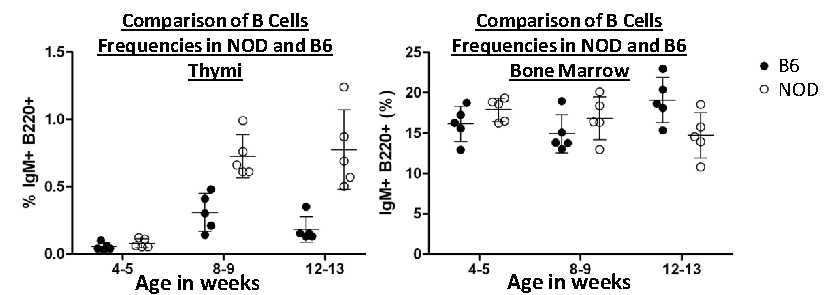
\includegraphics[width=\textwidth]{Figures/JVgraph.pdf}
\caption{B cells increase in the NOD thymus but not bone marrow compared to B6 controls.
The increase is more pronounced as mice age}
\label{fig:JVgraph}
\end{figure}

The age-related increase in B cells is intriguing as it appears to correlate with the progression of the disease in the NOD mouse.
This could suggest that either thymic B cells are involved in driving the disease progression, or it may be that they are a result of disease progression.

This increase in thymic B cells is not entirely unique to NOD mice, it is also a phenomenon seen in other autoimmune diseases such as myasthenia gravis \citep{Vrolix2014, Christensson1988} and therefore unravelling the origin and function of thymic B cells in the NOD mouse, may have benefits beyond those in the field of T1D.


\subsubsection{Potential role of thymic B cells in T1D}

The function of thymic B cells is not known.
However, it is proposed that they may be interfering with the proces of negative selection as they have been seen to position themselves next to mTECs in the thymus.
This would fit with the fact that the thymic B cell population increases as the disease progresses.
The increase in thymic B cells may be related to the increasing release of autoreactive T cells seen with disease progression.

\paragraph{Interference in negative selection}

There is evidence to suggest that B cells are able to take part in T cell negative selection, and it fact help to delete autoreactive T cells from the repertoire during development \citep{Frommer2010}.
This could suggest that B cells in the thymus are increased in response to a rising number of autoreactive T cells and are therefore trying to reduce the number of autoreactive T cells, rather than promoting their release.

It has also been found that B cells in the thymus, but not the periphery can express AIRE \citep{Yamano2015}, further suggesting that they may be involved in T cell negative selection.
However, it was also investigated as to whether these AIRE expressing B cells came from immigrating B cells or intrathymic development.
Splenic B cells were transferred to receipient mice and it was seen that one week after transfer, there were AIRE expressing donor cells in the thymus.
It appeared that B cells moving into the thymus were affected by something in the thymic environment which changed them to becoming AIRE+.

T1D is believed to be due, at least in part, to a breakdown in negative selection.
This coupled with increased population of B cells in the thymus, potentially capable of mediating negative selection could point to a number of links.
It may be that B cells are being upregulated in the thymus to tackle the increased population of autoreactive T cells.
Or it may be that B cells themselves are becoming dysregulated in the NOD thymus and instead of being helpful, they may be hindering the process of negative selection and actually promoting the release of autoreactive T cells.
It remains to be seen.

\section{Project Aims}

The aim of this project is to more fully understand the process of potential intrathymic development.
These are the main questions that this project aims to investigate:
\begin{itemize}
\item Is there presence of early progenitors, developing B cells and active development of B cells in the NOD thymus?
\item Does the thymus of the NOD WT mouse look different to NOD.$\mu$MT B cell KO mice in terms of B cell progenitors/developing B cells?
\item How does the NOD thymus compare to the nondiabetic B6 thymus in terms of intrathymic B cell development?
\end{itemize}

\begin{figure}
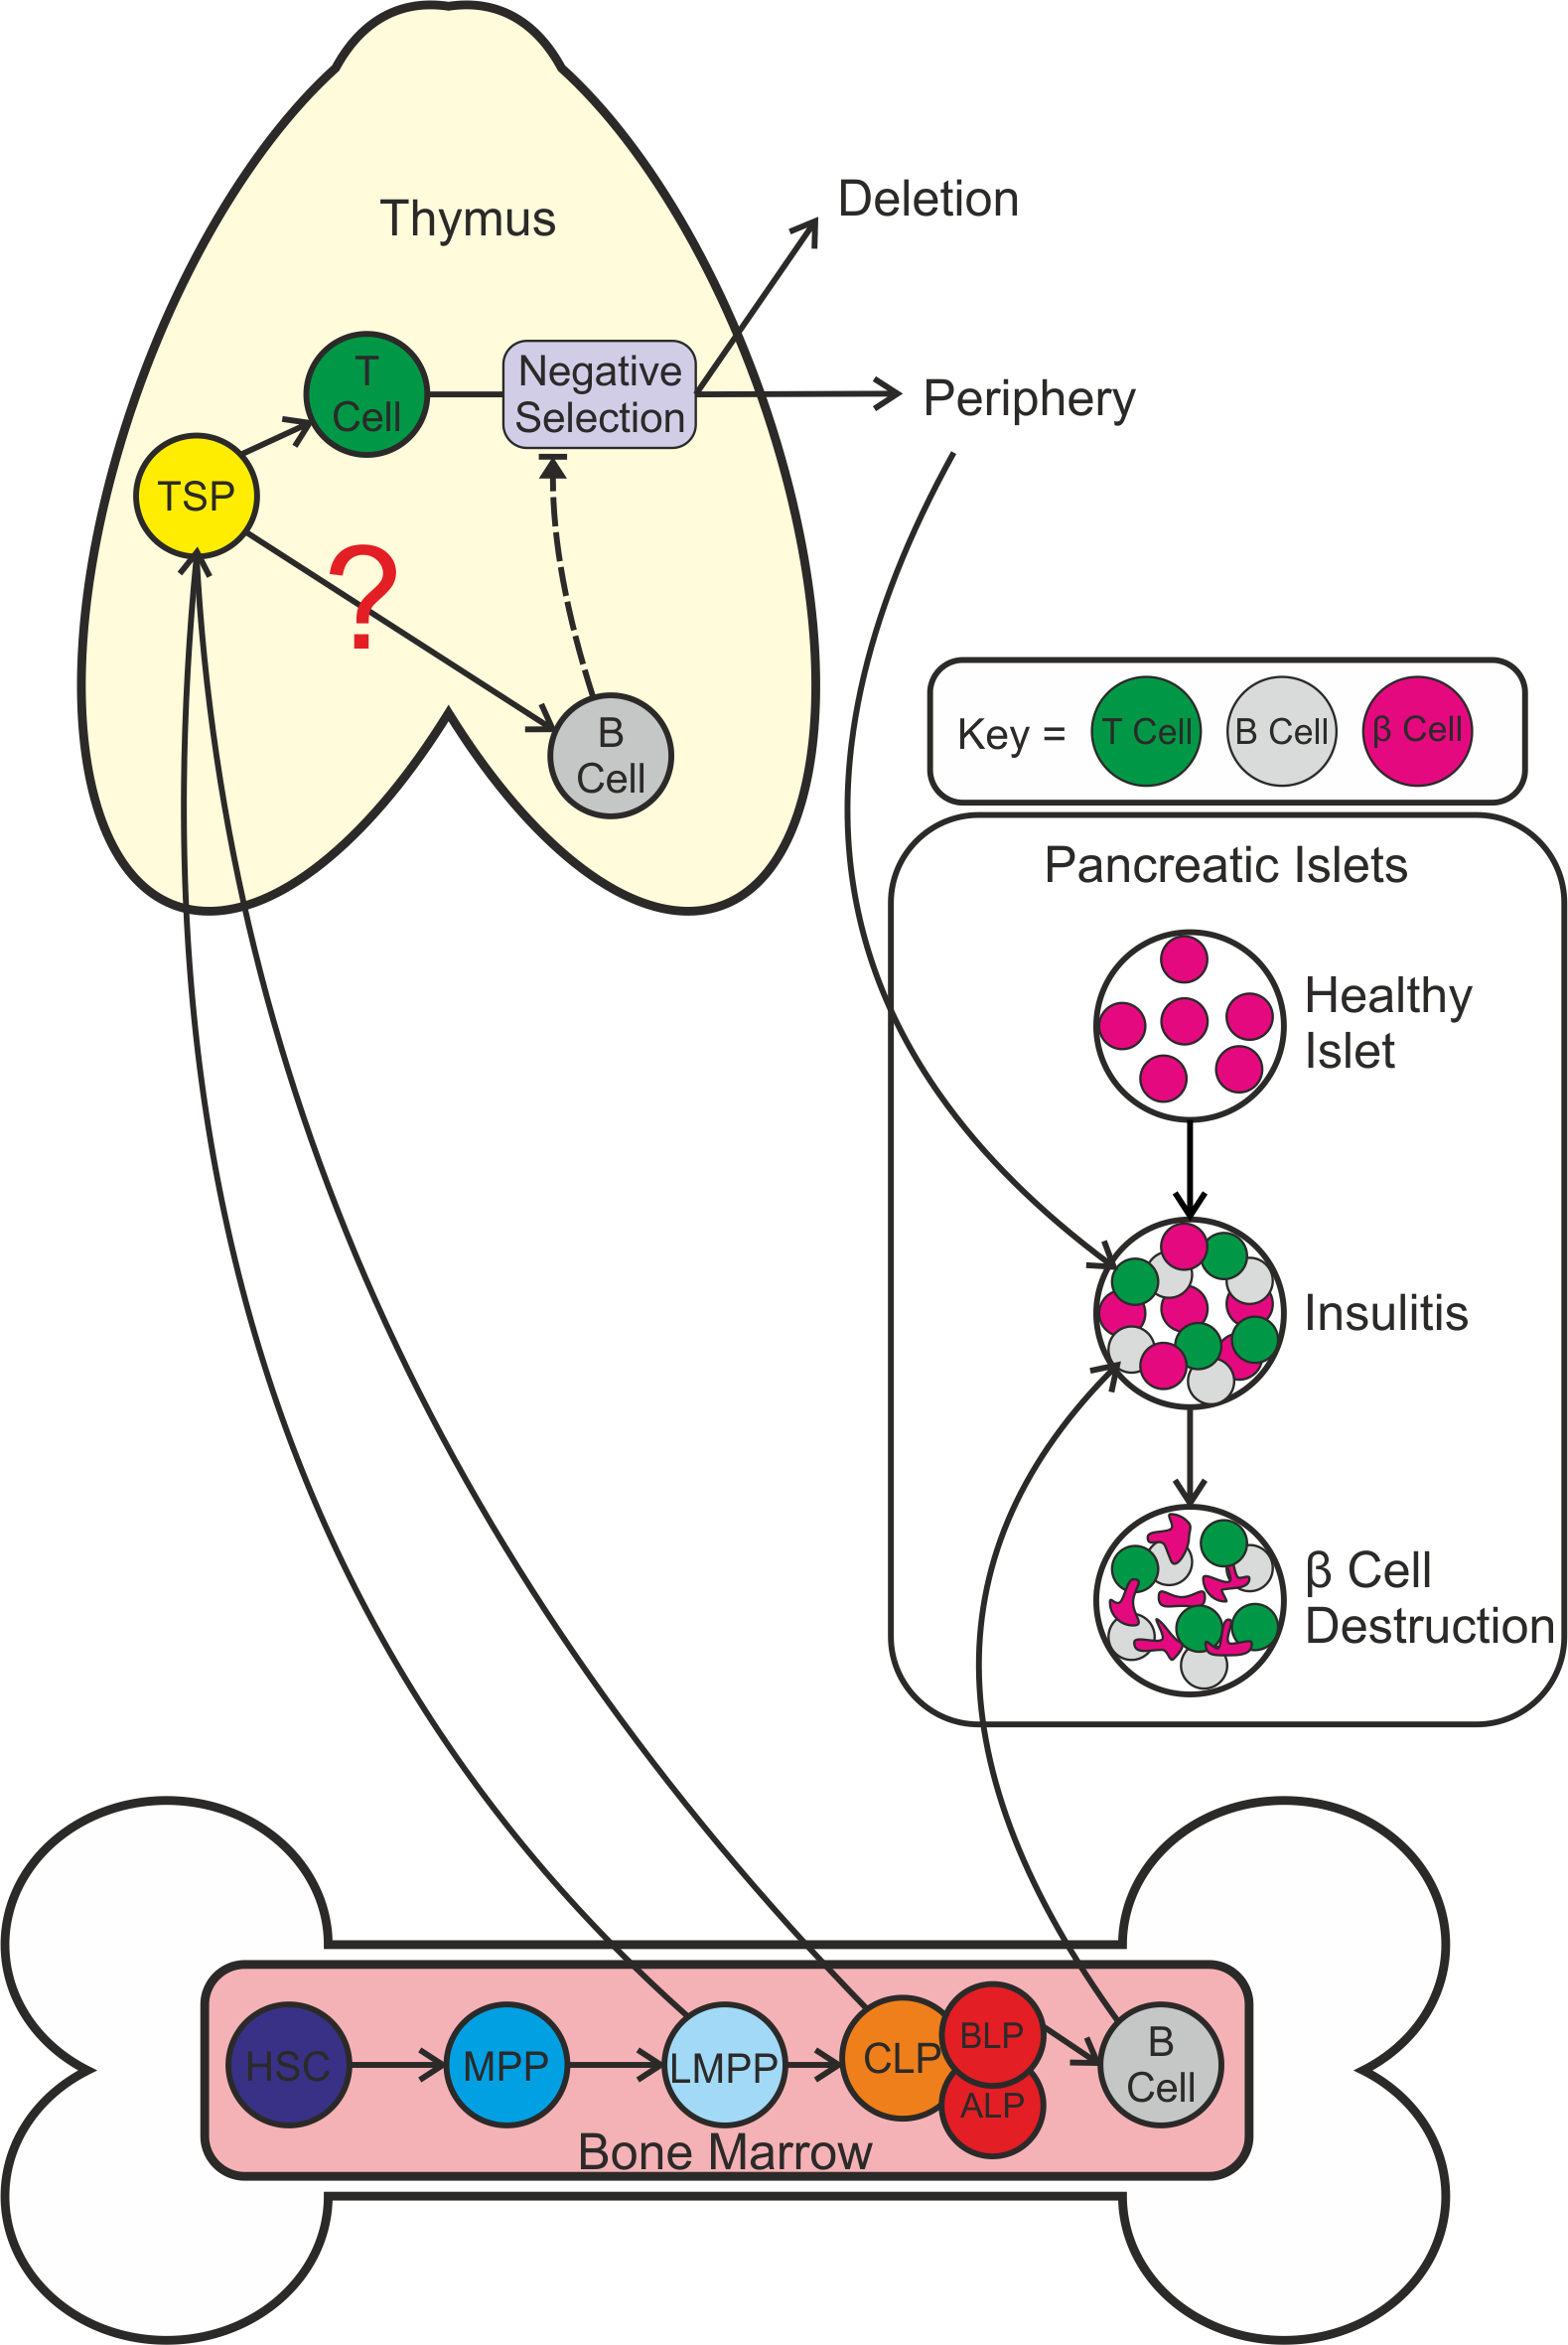
\includegraphics[width=\textwidth]{Figures/Introductorydiagram.png}
\caption{B cells develop in bone marrow, T cells develop in thymus. Are some progenitors in the thymus capable of producing B cells in the thymus?
In T1D, healthy islets become infiltrated with immune cells, including B and T cells, then $\beta$ cells are destroyed by CTLs.}
\label{fig:summarydiagram}
\end{figure}




































